\documentclass[11pt,a4paper]{ctexart}

\usepackage{geometry}
\usepackage{graphicx}
\usepackage{booktabs}
\usepackage{array}
\usepackage{amsmath}
\usepackage[hidelinks]{hyperref}
\usepackage{caption}
\usepackage{float}
\usepackage{tabularx}
\usepackage{enumitem}
\usepackage{fvextra}

\geometry{
  left=2.2cm,
  right=2.2cm,
  top=2.2cm,
  bottom=2.2cm
}

\graphicspath{{figures/}}
\captionsetup{font=small}
\setlength{\parindent}{2em}
\setlength{\parskip}{0.25em}
\renewcommand{\arraystretch}{1.15}
\setlist{nosep,leftmargin=2em}

\title{基于多模态大模型与 Skill 的肝脏超声包虫病识别探索}
\author{}
\date{}

\begin{document}

\maketitle

\section{任务与核心问题}

本项目完成了以下工作：

\begin{itemize}
    \item 构建包含 166 张图像的 liver ultrasound benchmark；
    \item 建立统一的 multimodal LLM Agent pipeline；
    \item 比较 GLM-5.3-Flash 与 DeepSeek-V4-Flash-Vision-Exp；
    \item 设计并迭代 Skill v1--v4；
    \item 冻结实验方案后，在 held-out test 上完成最终评估。
\end{itemize}

Skill 是附加在任务 prompt 中的文本判读流程，不是训练、微调或新的分类器。本项目的核心问题是：\textbf{额外 Skill 对不同基础多模态模型的影响是否一致？}

\section{数据与实验设计}

最终 benchmark 共 166 张图像，包括 83 张肝脏包虫病超声（positive）和 83 张非包虫病肝脏超声（negative）。negative 包含 Normal、Benign 和 Malignant，\textbf{不等于 healthy}。

\begin{center}
\begin{tabular}{lccc}
\toprule
Split & Positive & Negative & Total \\
\midrule
dev & 50 & 50 & 100 \\
held-out test & 33 & 33 & 66 \\
\bottomrule
\end{tabular}
\end{center}

dev 用于 Skill 设计迭代，held-out test 在开发过程中保持隔离。positive 与 negative 来自不同公开数据来源，因此存在 source/domain bias 风险。

两种模型使用相同的任务说明、数据划分、结构化输出和评估方式。实验流程为：

\begin{center}
\texttt{Image + task prompt + optional Skill}
$\rightarrow$ \texttt{Multimodal LLM}
$\rightarrow$ \texttt{structured prediction}
$\rightarrow$ \texttt{evaluation}
\end{center}

\section{Baseline 的不同错误画像}

在介绍 Skill 前，先比较两个模型在当前 held-out benchmark 上观察到的 baseline error pattern：

本文将包虫病图像定义为阳性（positive），非包虫病肝脏超声定义为阴性（negative）。图表中的缩写统一解释如下：

\begin{center}
\small
\begin{tabularx}{0.94\textwidth}{@{}>{\bfseries}p{1.4cm}p{5.6cm}X@{}}
\toprule
缩写 & 中英文名称 & 在本任务中的具体含义 \\
\midrule
TP & 真阳性 / True positive & 阳性图像被正确判断为包虫病 \\
FN & 假阴性 / False negative & 阳性图像被误判为阴性，即漏掉包虫病 \\
FP & 假阳性 / False positive & 阴性图像被误判为包虫病，即阳性误报 \\
TN & 真阴性 / True negative & 阴性图像被正确判断为非包虫病 \\
\bottomrule
\end{tabularx}
\end{center}

Accuracy（准确率）为全部样本中判断正确的比例；Sensitivity（灵敏度）为阳性样本中被正确识别的比例，即 $TP/(TP+FN)$；Specificity（特异度）为阴性样本中被正确识别的比例，即 $TN/(TN+FP)$。

\begin{center}
\small
\begin{tabular}{lrrrrr}
\toprule
Model & 准确率 & 灵敏度 & 特异度 & FN（假阴性） & FP（假阳性） \\
\midrule
GLM baseline & 93.94\% & 87.88\% & 100.00\% & 4 & 0 \\
DeepSeek baseline & 71.21\% & 96.97\% & 45.45\% & 1 & 18 \\
\bottomrule
\end{tabular}
\end{center}

在当前 test 上，GLM baseline 的 FP 为 0，主要剩余错误是 FN；DeepSeek baseline 的 FN 很少，但存在大量 FP，即明显的阳性过判。两个基础模型在加入 Skill 前面对的主要问题已经不同。这里描述的是当前 benchmark 上的观察结果，不代表模型在其他数据上的固定特征。

\section{Skill v1--v4 的设计迭代}

Skill 的设计迭代逻辑是：根据上一版本在 dev 上观察到的问题，设计下一版本进行检验；当前实验不据此建立严格因果关系。

\begin{table}[H]
\centering
\small
\begin{tabularx}{\textwidth}{@{}>{\bfseries}p{1.5cm}p{4.8cm}X@{}}
\toprule
Version & 核心设计 & 观察与下一步 \\
\midrule
v1 & 显式 CE morphology checklist，并强调避免过度诊断 & GLM sensitivity 明显下降，表现过于保守；下一步放宽强排除条件 \\
v2 & 放宽 checklist 中的强排除条件，减少不必要拒判 & sensitivity 仍未恢复，说明问题不只是个别措辞；下一步移除长疾病 checklist \\
v3 & 仅保留 systematic observation 与 evidence integration & GLM dev 恢复到 baseline 附近；DeepSeek FP 明显减少；下一步检验示例化 evidence integration \\
v4 & v3 加入 worked reasoning example & 检验示例是否进一步有效；最终效果仍表现出 model dependence \\
\bottomrule
\end{tabularx}
\caption{Skill v1--v4 的设计迭代逻辑。}
\label{tab:skill_iteration}
\end{table}

GLM 在同一 dev100 上的严格准确率为：baseline 85\%、v1 78\%、v2 77\%、v3 85\%。这组结果解释了为什么从显式 checklist 转向更精简的结构化观察流程。DeepSeek dev100 的 FP 在 baseline 与 v3 间由 34 降至 24。

v4 的 worked example 来源于 dev 中一张图像的 source-provided morphology description，因此该样本未计入 v4 的开发集评估；v4 使用 99 张的公平评估集合，详细说明见附录。

\section{Held-out test 最终结果}

最终评估使用固定的 66 张 held-out test（33 positive、33 negative）。六个条件覆盖相同图像，均无 \texttt{not\_applicable} 或解析失败。

\begin{figure}[H]
    \centering
    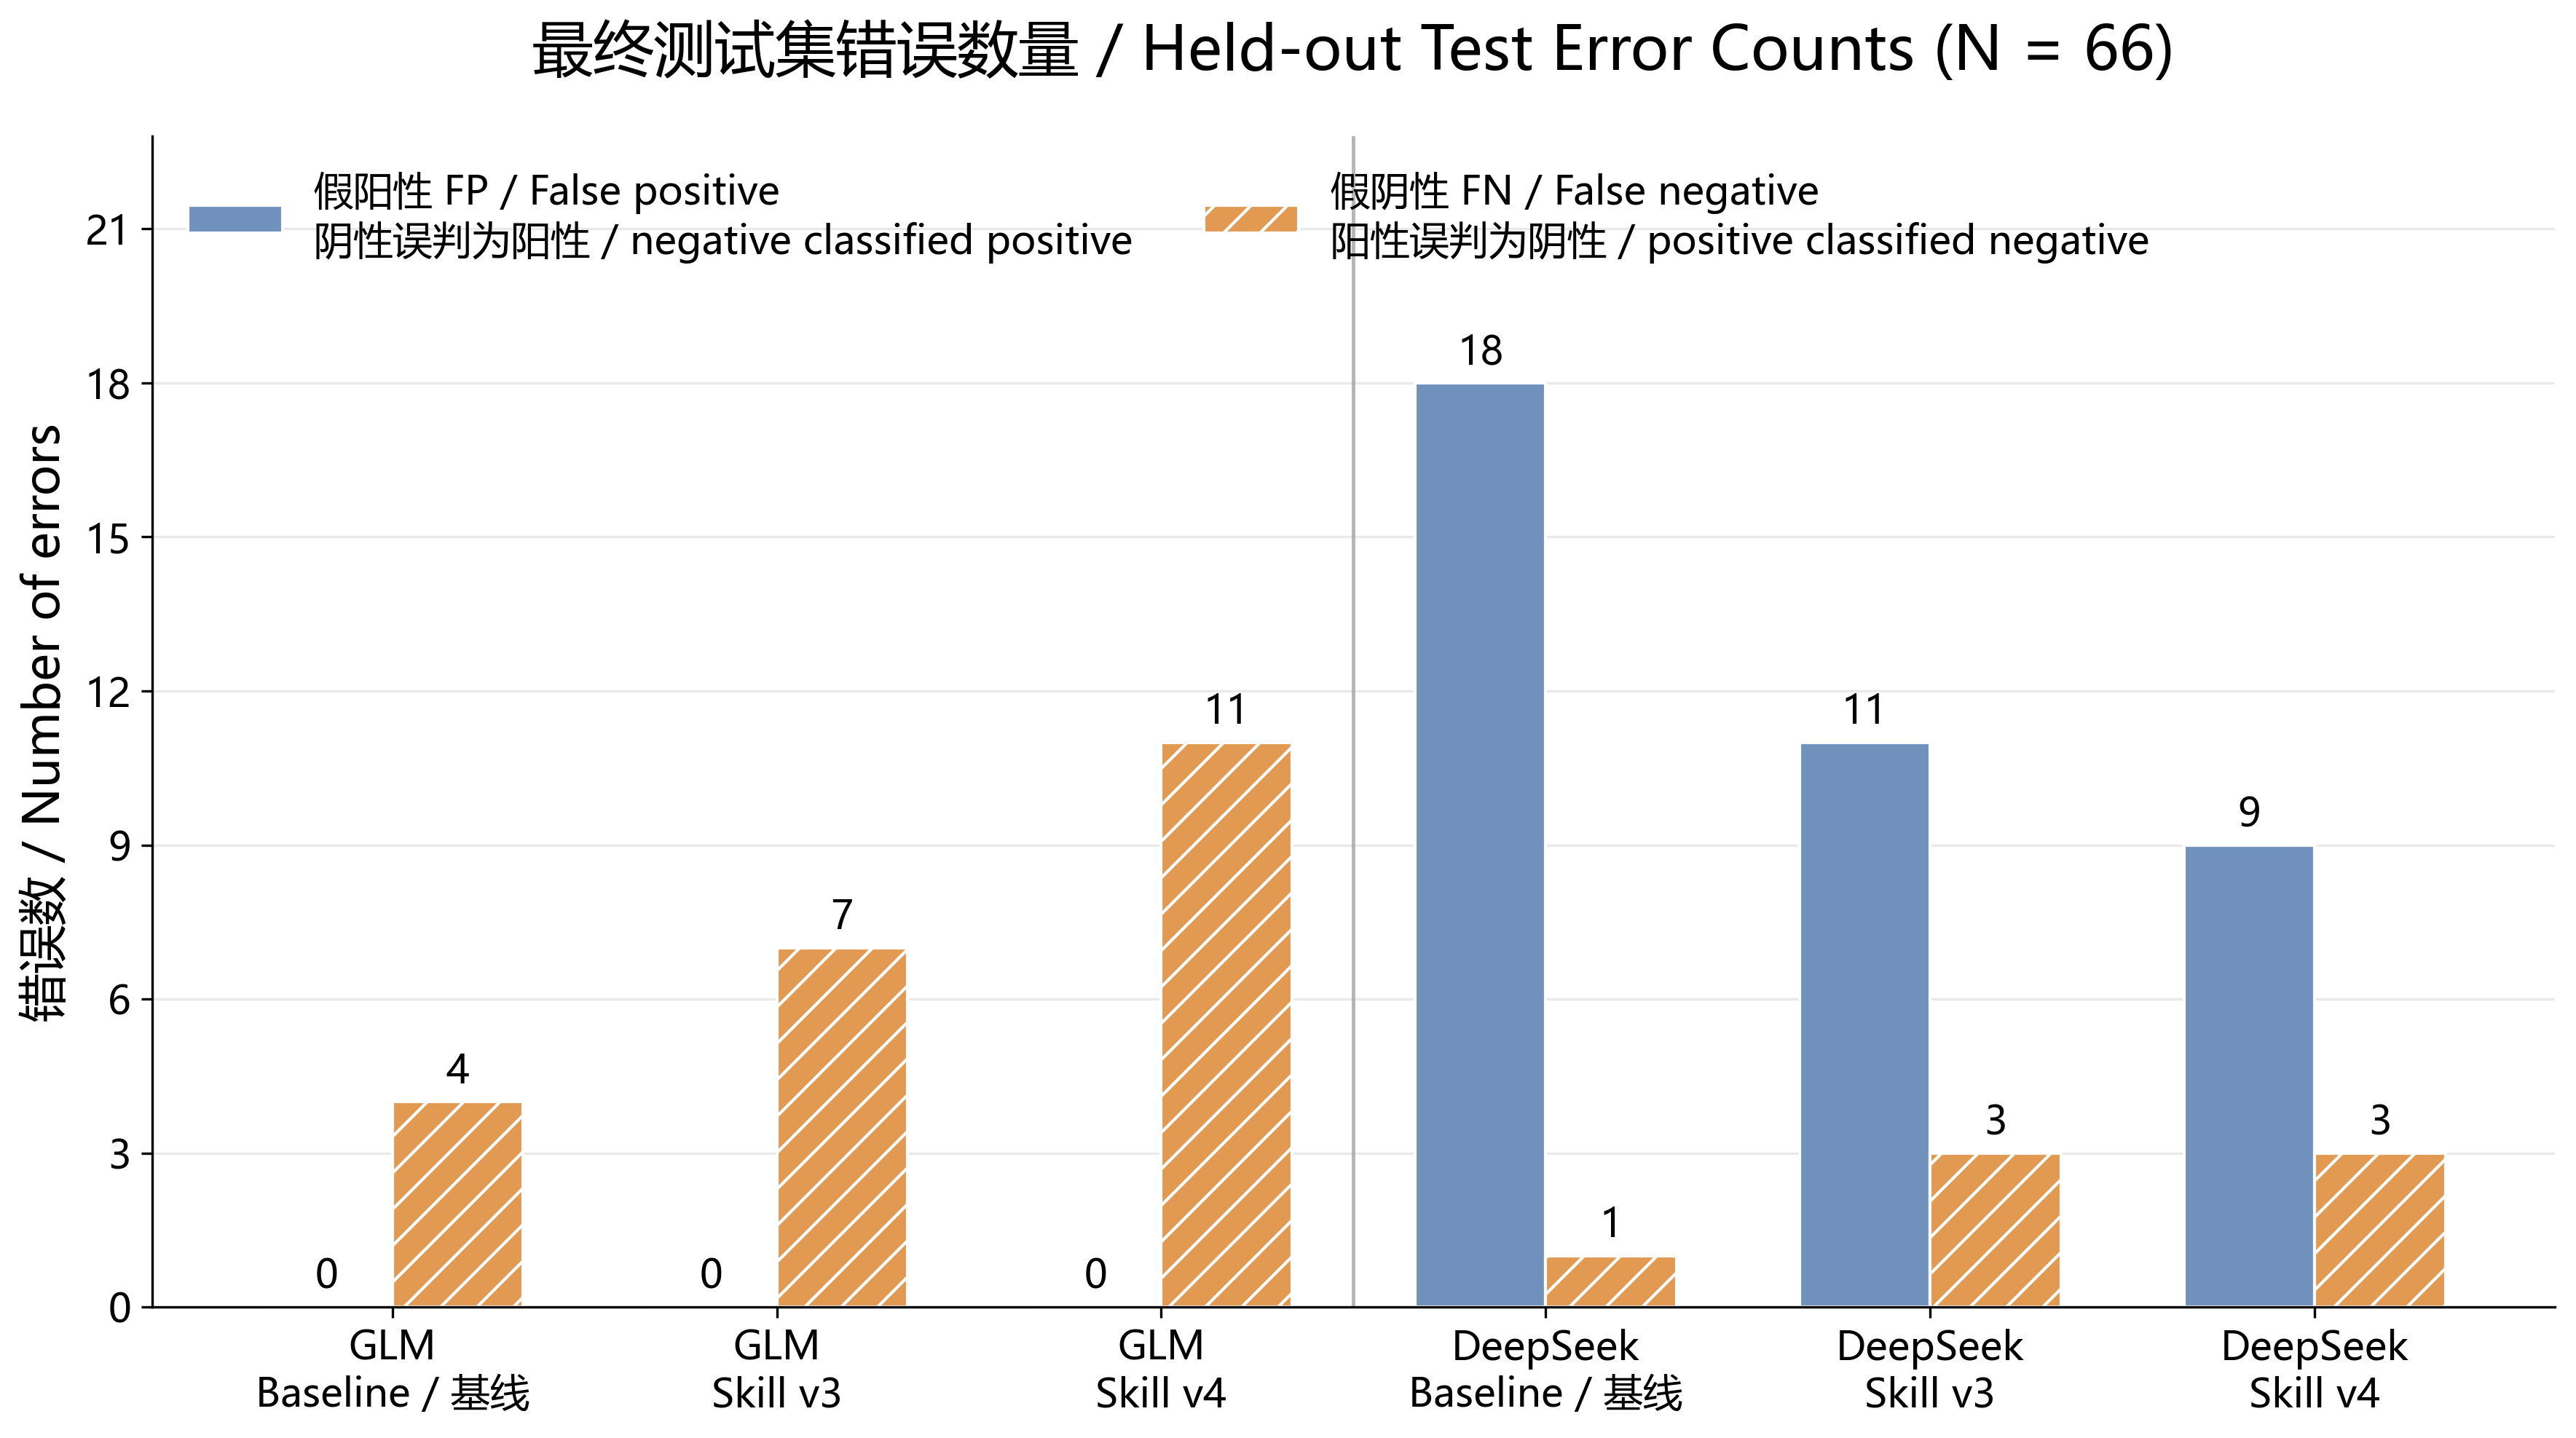
\includegraphics[width=0.84\textwidth]{fig02_error_counts.png}
    \caption{Held-out test 错误数量。FP（假阳性）表示阴性被误判为阳性；FN（假阴性）表示阳性被误判为阴性。}
    \label{fig:error_counts}
\end{figure}

图~\ref{fig:error_counts} 直接展示了核心现象：在 v3/v4 条件下，两种模型都观察到阳性预测倾向下降，但由于 baseline error pattern 不同，产生了不同的 error trade-off。

\begin{table}[H]
\centering
\small
\resizebox{\textwidth}{!}{%
\begin{tabular}{@{}llrrrrrrr@{}}
\toprule
Model & Condition & \shortstack{TP\\真阳性} & \shortstack{FN\\假阴性} & \shortstack{FP\\假阳性} & \shortstack{TN\\真阴性} & 准确率 & 灵敏度 & 特异度 \\
\midrule
GLM & baseline & 29 & 4 & 0 & 33 & 93.94\% & 87.88\% & 100.00\% \\
GLM & Skill v3 & 26 & 7 & 0 & 33 & 89.39\% & 78.79\% & 100.00\% \\
GLM & Skill v4 & 22 & 11 & 0 & 33 & 83.33\% & 66.67\% & 100.00\% \\
DeepSeek & baseline & 32 & 1 & 18 & 15 & 71.21\% & 96.97\% & 45.45\% \\
DeepSeek & Skill v3 & 30 & 3 & 11 & 22 & 78.79\% & 90.91\% & 66.67\% \\
DeepSeek & Skill v4 & 30 & 3 & 9 & 24 & 81.82\% & 90.91\% & 72.73\% \\
\bottomrule
\end{tabular}%
}
\caption{六个条件在 held-out test 上的主要指标。}
\label{tab:test_results}
\end{table}

\textbf{GLM：}FN 从 4 增至 7、11，FP 始终为 0。在当前 test 上，GLM baseline 已经没有 FP；v3/v4 没有带来额外 specificity 收益，主要增加 FN，使 sensitivity 和 accuracy 下降。

\textbf{DeepSeek：}FP 从 18 降至 11、9，FN 从 1 增至 3 后保持不变。v3/v4 主要减少 FP，同时带来少量 FN 增加，因此 specificity 与 overall accuracy 上升，sensitivity 略有下降。

\begin{figure}[H]
    \centering
    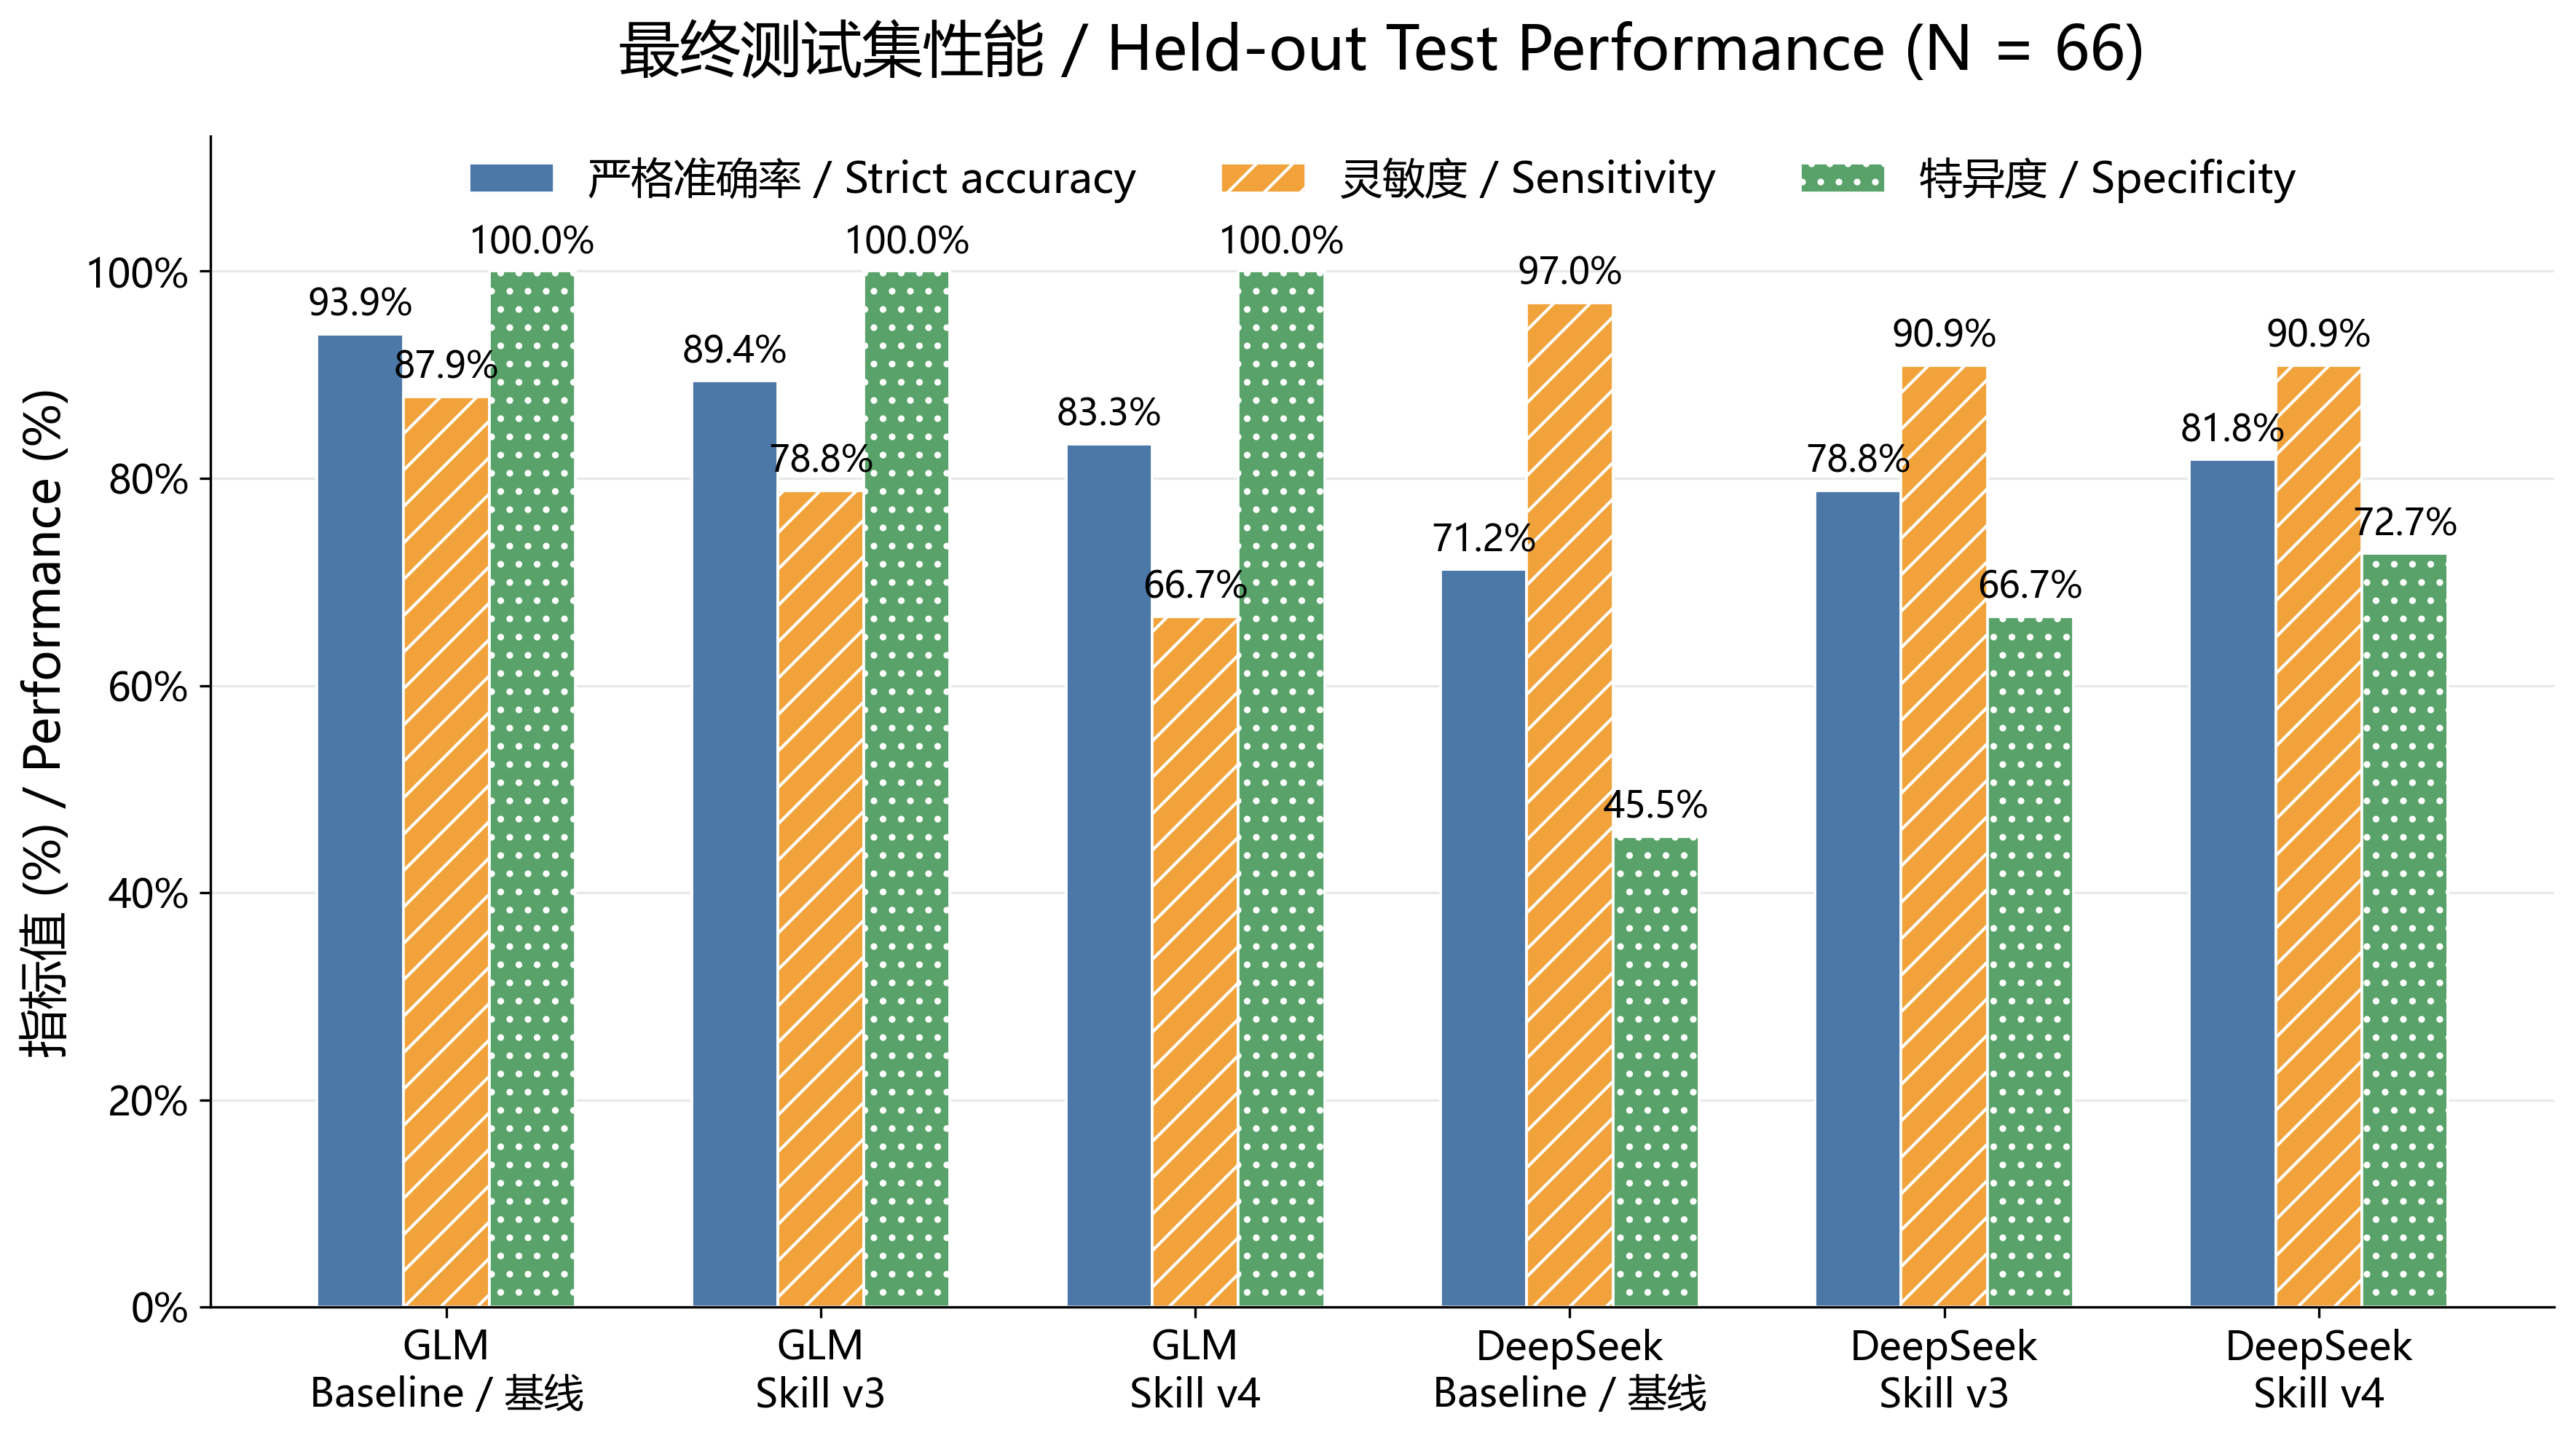
\includegraphics[width=0.90\textwidth]{fig01_test_performance.png}
    \caption{六个 held-out test 条件的严格准确率（Strict accuracy）、灵敏度（Sensitivity）与特异度（Specificity）。}
    \label{fig:test_performance}
\end{figure}

图~\ref{fig:test_performance} 从比例指标上补充显示：GLM 的主要变化是 sensitivity 下降；DeepSeek 的主要变化是 specificity 上升。

\section{核心发现、局限与下一步}

\subsection{三个核心发现}

\begin{enumerate}
    \item \textbf{Skill 不是普遍增益。} 在当前 benchmark 上，GLM baseline 优于其 Skill 条件，而 DeepSeek 的 observed accuracy 在 v3/v4 下提高。
    \item \textbf{Skill 更像改变模型的 observed decision behavior。} 主要表现为 sensitivity--specificity trade-off，而不能简单解释为“增加了医学知识”。
    \item \textbf{Skill 效果依赖基础模型原本的 error pattern。} 两个 baseline 面对的主要错误不同，阳性预测倾向下降因而产生不同后果。
\end{enumerate}

\begin{center}
\small
\begin{tabular}{lccc}
\toprule
Comparison & FP & FN & Accuracy \\
\midrule
GLM baseline $\rightarrow$ v4 & $0\rightarrow0$ & $4\rightarrow11$ & $93.94\%\rightarrow83.33\%$ \\
DeepSeek baseline $\rightarrow$ v4 & $18\rightarrow9$ & $1\rightarrow3$ & $71.21\%\rightarrow81.82\%$ \\
\bottomrule
\end{tabular}
\end{center}

因此，同样表现为“阳性预测倾向下降”的提示变化，在 DeepSeek 上主要修正 false positives，但在 GLM 上主要增加 false negatives。worked reasoning example 也没有表现出跨模型一致收益：相对 v3，v4 在 GLM 上降低 accuracy，在 DeepSeek 上提高 accuracy。

DeepSeek baseline vs v4 的 McNemar exact $p=0.092285$，因此当前结果不能表述为 statistically significant improvement。

\subsection{主要局限}

\begin{itemize}
    \item 数据规模较小，且只使用一个固定 dev/test split；
    \item positive 与 negative 来自不同公开来源，存在 source/domain bias；
    \item 输入为单张静态 ultrasound，缺少完整临床信息和独立医生复核。
\end{itemize}

本实验属于 exploratory / pilot benchmark，不能用于推断真实临床诊断性能。

\subsection{下一步讨论}

\begin{enumerate}
    \item 是否需要构建来源匹配的 positive/negative 数据，或设置独立外部 test？
    \item 是否应扩大到多中心、多设备和更多图像，进一步纳入多帧或动态超声？
    \item 下一步 Skill 是否仍应聚焦 prompt-level reasoning，还是转向 multi-stage agent / tool-assisted workflow？
\end{enumerate}

\section*{附录 / 补充结果}
\addcontentsline{toc}{section}{附录 / 补充结果}

\subsection*{完整 held-out test 指标}

\begin{center}
\scriptsize
\resizebox{\textwidth}{!}{%
\begin{tabular}{llrrrrrrrrrrrr}
\toprule
Model & Condition & N & TP & FN & FP & TN & NA & PF & Accuracy & Precision & Sensitivity & Specificity & F1 \\
\midrule
GLM & baseline & 66 & 29 & 4 & 0 & 33 & 0 & 0 & 93.94\% & 100.00\% & 87.88\% & 100.00\% & 93.55\% \\
GLM & Skill v3 & 66 & 26 & 7 & 0 & 33 & 0 & 0 & 89.39\% & 100.00\% & 78.79\% & 100.00\% & 88.14\% \\
GLM & Skill v4 & 66 & 22 & 11 & 0 & 33 & 0 & 0 & 83.33\% & 100.00\% & 66.67\% & 100.00\% & 80.00\% \\
DeepSeek & baseline & 66 & 32 & 1 & 18 & 15 & 0 & 0 & 71.21\% & 64.00\% & 96.97\% & 45.45\% & 77.11\% \\
DeepSeek & Skill v3 & 66 & 30 & 3 & 11 & 22 & 0 & 0 & 78.79\% & 73.17\% & 90.91\% & 66.67\% & 81.08\% \\
DeepSeek & Skill v4 & 66 & 30 & 3 & 9 & 24 & 0 & 0 & 81.82\% & 76.92\% & 90.91\% & 72.73\% & 83.33\% \\
\bottomrule
\end{tabular}%
}
\end{center}

六个条件均无拒判或解析失败，因此 Overall Accuracy 与 Strict Accuracy 相同。

\subsection*{McNemar exact test}

\begin{center}
\small
\begin{tabular}{llrrr}
\toprule
Model & Comparison & correct$\rightarrow$wrong & wrong$\rightarrow$correct & Exact two-sided $p$ \\
\midrule
GLM & baseline vs v3 & 6 & 3 & 0.507812 \\
GLM & baseline vs v4 & 8 & 1 & 0.039062 \\
GLM & v3 vs v4 & 7 & 3 & 0.343750 \\
DeepSeek & baseline vs v3 & 3 & 8 & 0.226562 \\
DeepSeek & baseline vs v4 & 3 & 10 & 0.092285 \\
DeepSeek & v3 vs v4 & 4 & 6 & 0.753906 \\
\bottomrule
\end{tabular}
\end{center}

GLM baseline vs v4 的差异主要体现为 sensitivity 下降。DeepSeek baseline vs v3/v4 均未达到传统 $p<0.05$ 阈值；统计证据也不等同于临床意义。

\subsection*{三类阴性来源的分类正确率}

33 张 test 阴性样本包括 Normal（正常）5 张、Benign（良性病变）9 张和 Malignant（恶性病变）19 张。本节的“分类正确率”专指每一类阴性样本中被正确判断为阴性的比例，即 $TN/N$；它等价于该阴性来源类别内部的 specificity，不是整个 test 的 overall accuracy。

\begin{center}
\small
\begin{tabular}{llrrr}
\toprule
Model & Condition & Normal（$n=5$） & Benign（$n=9$） & Malignant（$n=19$） \\
\midrule
GLM & baseline & 5/5（100.00\%） & 9/9（100.00\%） & 19/19（100.00\%） \\
GLM & Skill v3 & 5/5（100.00\%） & 9/9（100.00\%） & 19/19（100.00\%） \\
GLM & Skill v4 & 5/5（100.00\%） & 9/9（100.00\%） & 19/19（100.00\%） \\
DeepSeek & baseline & 3/5（60.00\%） & 5/9（55.56\%） & 7/19（36.84\%） \\
DeepSeek & Skill v3 & 4/5（80.00\%） & 4/9（44.44\%） & 14/19（73.68\%） \\
DeepSeek & Skill v4 & 4/5（80.00\%） & 6/9（66.67\%） & 14/19（73.68\%） \\
\bottomrule
\end{tabular}
\end{center}

\begin{figure}[H]
    \centering
    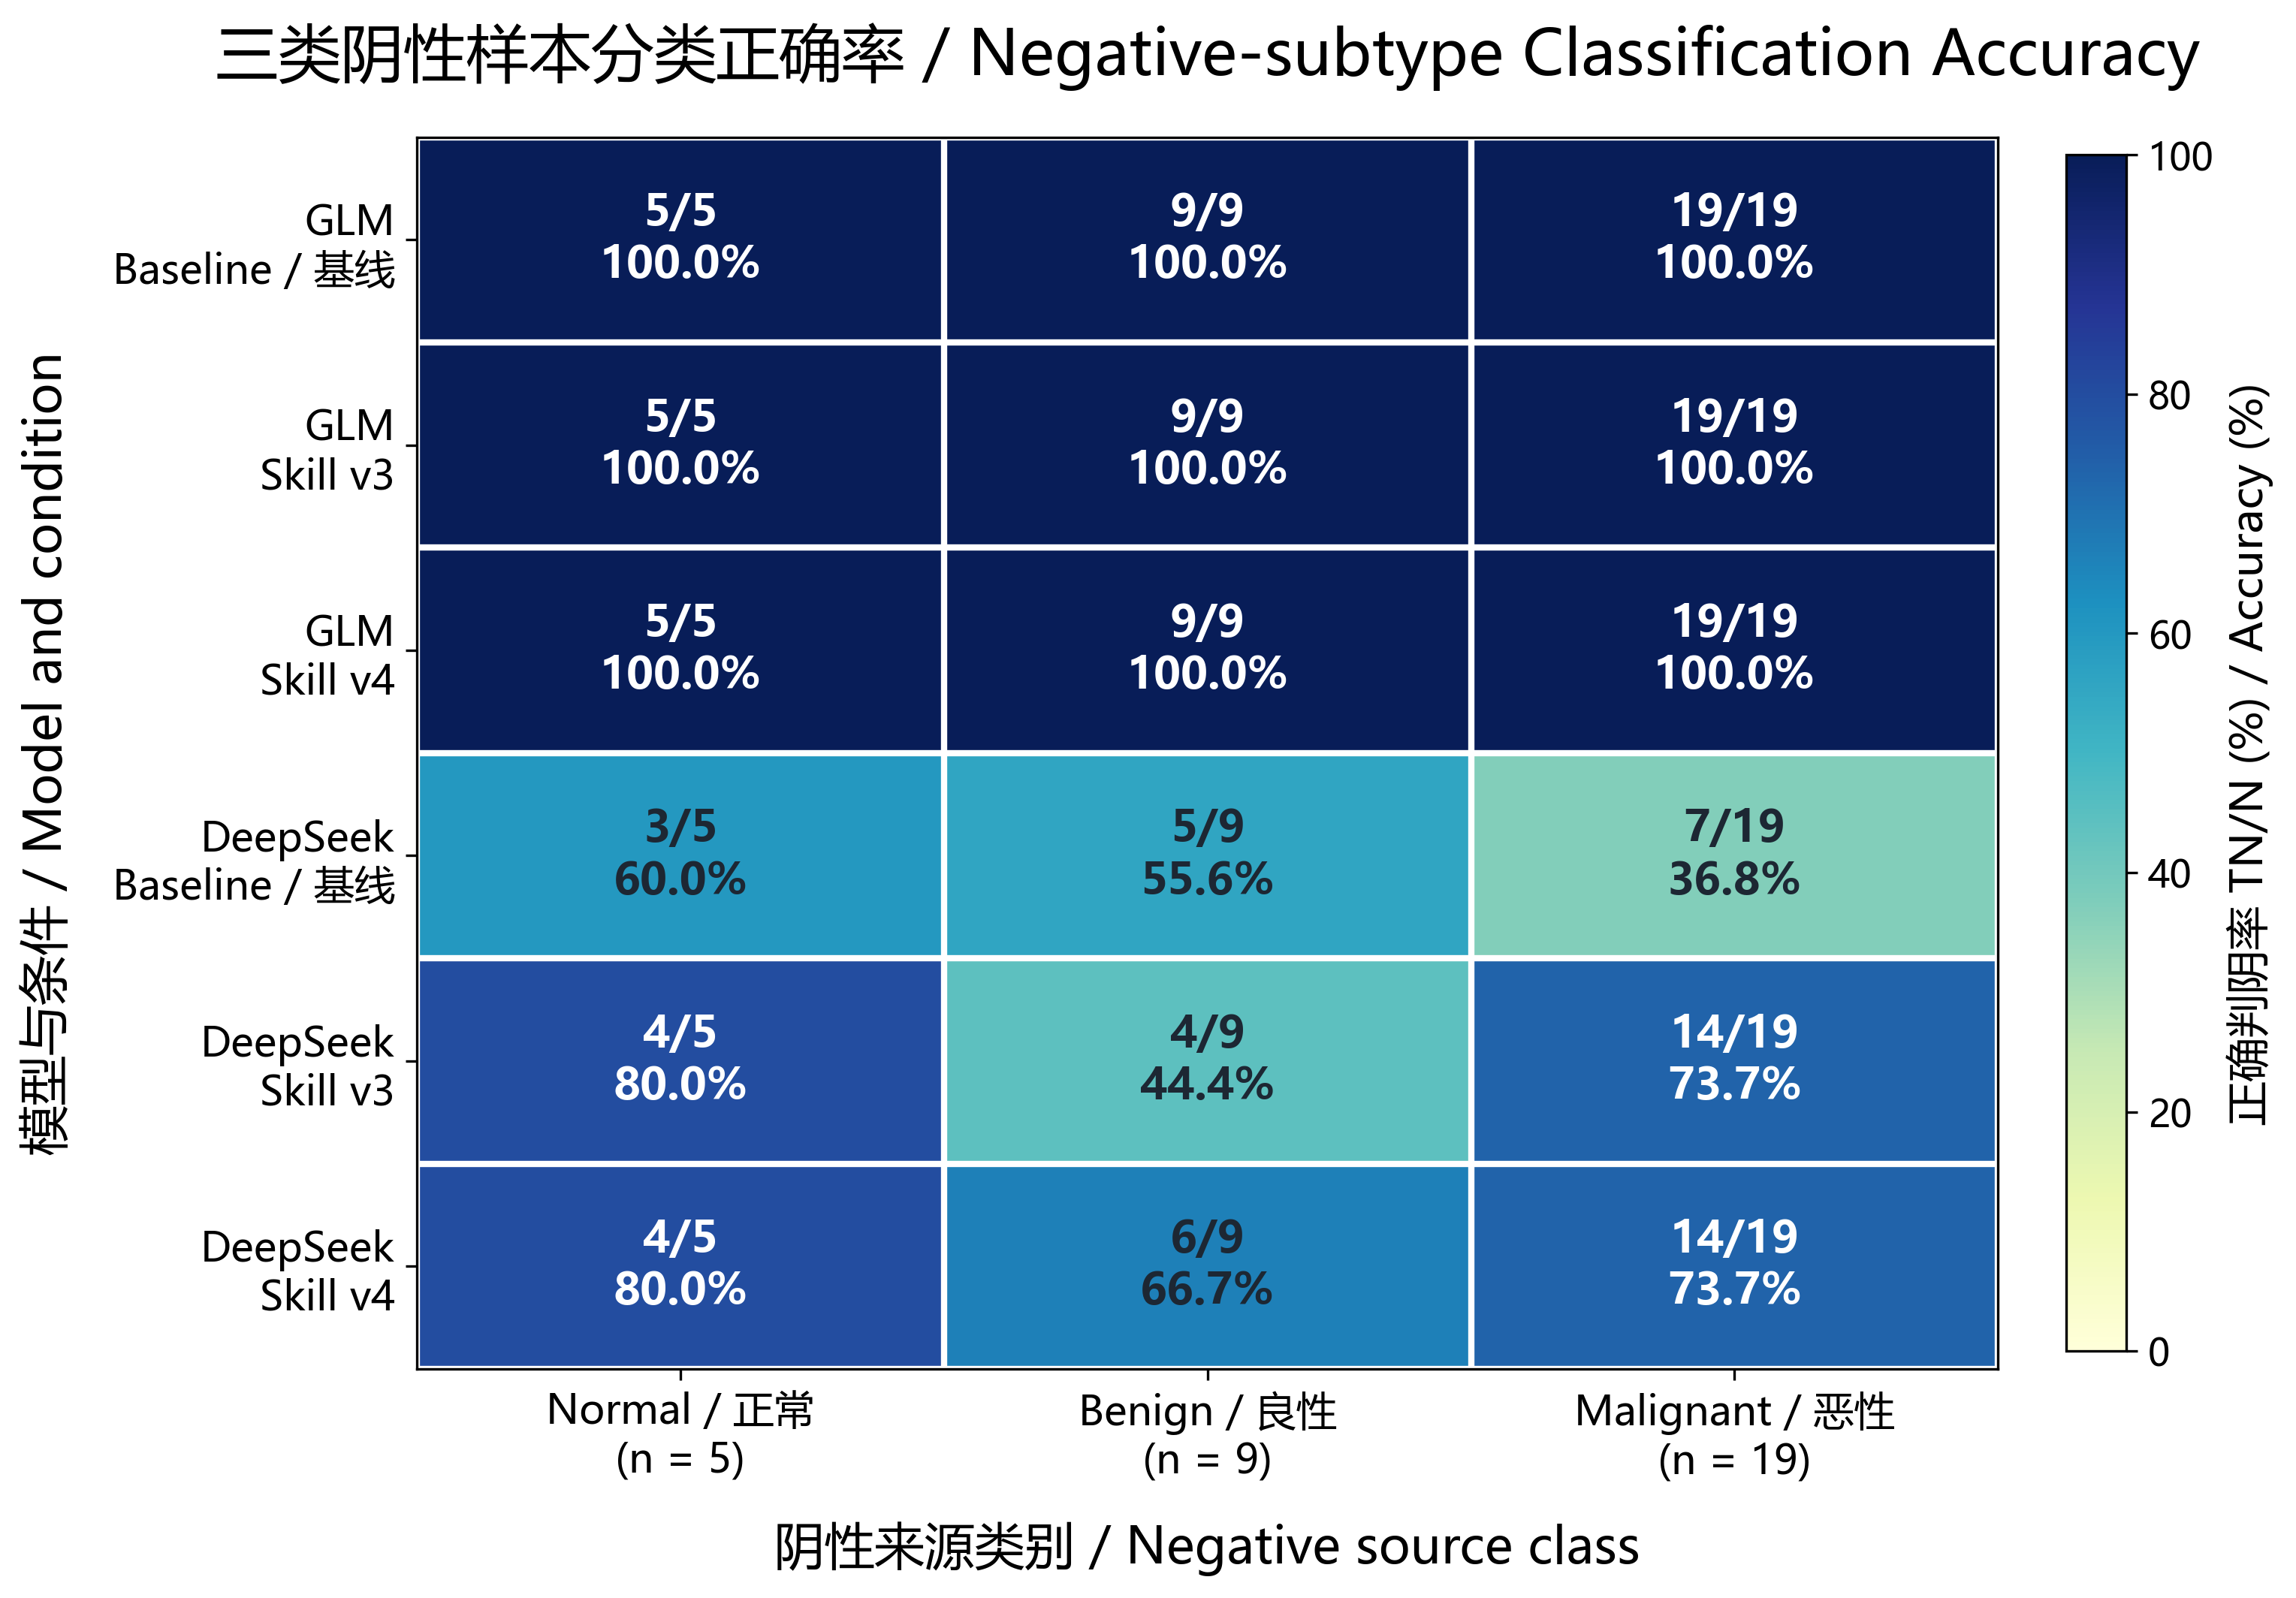
\includegraphics[width=0.86\textwidth]{fig03_deepseek_subtype_fpr.png}
    \caption{六种模型/Skill 条件在三类阴性来源上的分类正确率。每个单元格同时给出正确数/样本数与百分比。}
    \label{fig:subtype_accuracy}
\end{figure}

GLM 的三种条件在三类阴性来源上均为 100\%，与其整体 FP 始终为 0 一致，因此 Skill 在当前 test 上没有额外改善 GLM 阴性分类的空间。DeepSeek baseline 在三类阴性来源上均有误报，其中 Malignant 最低，为 7/19（36.84\%）；v3/v4 均将 Malignant 提高到 14/19（73.68\%），Normal 从 3/5（60.00\%）提高到 4/5（80.00\%）。Benign 的变化不单调：baseline、v3、v4 分别为 55.56\%、44.44\% 和 66.67\%。因此，DeepSeek 的 FP 减少主要来自部分阴性来源类别，并非所有类别在每个版本中都同步改善。

该分层样本很小，尤其 Normal 仅 5 张、Benign 仅 9 张；以上结果只用于描述当前数据上的模型行为，不能据此提出新的医学结论。

\subsection*{v4 的 dev99 评估说明}

v4 的 worked reasoning example 由 dev 中 \texttt{img\_0020.jpg} 的 source-provided morphology description 抽象改写而来。为避免该信息影响开发集评估，该图像未计入 v4 评估，形成 \texttt{dev\_v4\_eval99}（49 positive、50 negative）；原始 dev100 和 held-out test 均未修改。

在同一 99 张集合上的公平比较如下：

\begin{center}
\small
\begin{tabular}{lrrr}
\toprule
Model & baseline & Skill v3 & Skill v4 \\
\midrule
GLM & 85.86\% & 85.86\% & 82.83\% \\
DeepSeek & 62.63\% & 69.70\% & 71.72\% \\
\bottomrule
\end{tabular}
\end{center}

这些 dev 结果只用于说明 Skill 设计迭代过程，最终泛化判断以冻结的 held-out test 为准。

\subsection*{Skill v1--v4 完整提示文本}

以下内容按冻结的 \texttt{SKILL.md} 原文呈现，并保留元数据头。它们是在统一 task prompt 之外附加给模型的完整 Skill 文本；baseline 不包含这些附加内容。

\subsubsection*{Skill v1}

\VerbatimInput[fontsize=\scriptsize,breaklines=true,breakanywhere=true]{appendix/skill_v1_prompt.txt}

\subsubsection*{Skill v2}

\VerbatimInput[fontsize=\scriptsize,breaklines=true,breakanywhere=true]{appendix/skill_v2_prompt.txt}

\subsubsection*{Skill v3}

\VerbatimInput[fontsize=\scriptsize,breaklines=true,breakanywhere=true]{appendix/skill_v3_prompt.txt}

\subsubsection*{Skill v4}

\VerbatimInput[fontsize=\scriptsize,breaklines=true,breakanywhere=true]{appendix/skill_v4_prompt.txt}

\end{document}
